\section{박종환 교수님 발표자료 검토}

본 절에서는 박종환 교수님의 발표자료를 검토한다. 먼저 발표자료에서 제공하는 KEM
구조를 설명한다. 여기서는 전부 내 생각이므로, 따로 메모를 적지 않으며, 지금까지
사용한 기호가 다를 수도 있음에 주의한다.

\subsection{Structure}

\newcommand{\ENCODE}{\textsf{Encode}}
\newcommand{\DECODE}{\textsf{Decode}}
\newcommand{\IDENT}{\textsf{Ident}}
\newcommand{\ENC}{\textsf{Enc}}
\newcommand{\DEC}{\textsf{Dec}}

% \begin{itemize}
% 	\item $\cK(1^{\lm})$: $(\pk, \sk)$를 생성한다. $\pk$는 이후 트랩도어 치환
% 	$\cF$에서 사용하며, $\sk$는 $\cI$에서 사용한다.
% 	\item $\cE_{\pk}(m; r)$: $m \in \bset^{n}$과 $r \rgets \bset^{\lm_0}$가
% 	주어졌을 때, $s, t$를 다음과 같이 계산한다.
% 	$$
% 		s = (m \parallel 0^{\lm_1}) \xor G(r), \quad
% 		t = r \xor H(s).
% 	$$
% 	$s, t$를 계산하는 과정을 도식화하면 그림 \ref{fig:oaep}와 같다. 이후 암호문 $c
% 	= \cF_{\pk}(s, t)$를 출력한다.
%   \item $\cD_{\sk}(c)$: $(s,t) = \cI_{\sk}(c)$을 계산한 후, $r, M$을 다음과 같이
%   계산한다.
% 	$$
%     	r = t \xor H(s), \quad M = s \xor G(r).
% 	$$
%   	만약 $[M]_{\lm_1} = 0^{\lm_1}$이면 $[M]^{n}$을 출력하고, 아니라면
%   	“$\textsf{Reject}$”를 출력한다. 이 때, $[M]_{\lm_1}$은 $M$의 마지막 $\lm_1$
%   	비트(LSB)를 의미하고, $[M]^{n}$은 $M$의 첫 $n$ 비트(MSB)를 의미한다.
% \end{itemize}

\begin{minipage}[t]{0.48\textwidth}
	\centering
	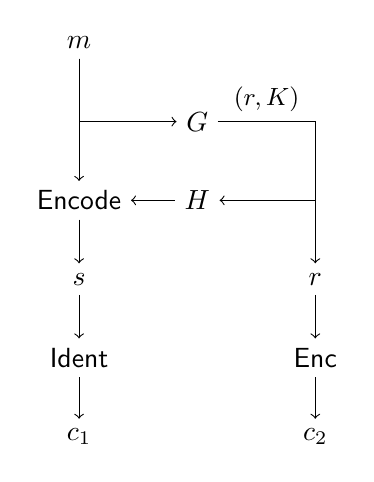
\begin{tikzpicture}
		\node (m) at (0, 0) {$m$};
		\node (G) at (1.5, -1) {$G$};
		\node (H) at (1.5, -2) {$H$};
		\node (s) at (0, -3) {$s$};
		\node (r) at (3, -3) {$r$};
		\node (Encode) at (0, -2) {$\ENCODE$};
		\node (Identity) at (0, -4) {$\IDENT$};
		\node (Enc) at (3, -4) {$\ENC$};
		\node (c1) at (0, -5) {$c_1$};
		\node (c2) at (3, -5) {$c_2$};

		\draw[->] (m) -- (Encode);
		\draw[->] (m) |- (G);
		\draw[->] (Encode) -- (s);
		\draw[->] (G) -| (r);
		\draw[->] (G) -- (3, -1) node[midway, above, font=\small] {$(r, K)$} -- (3, -2) -- (H);
		\draw[->] (H) -- (Encode);
		\draw[->] (s) -- (Identity);
		\draw[->] (r) -- (Enc);
		\draw[->] (Identity) -- (c1);
		\draw[->] (Enc) -- (c2);
	\end{tikzpicture}
	\captionof{figure}{Encapsulation}
	\label{fig:oaep_encap}
\end{minipage}
\hfill
\begin{minipage}[t]{0.48\textwidth}
	\centering
	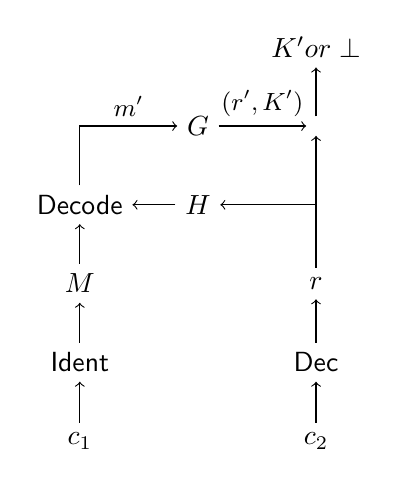
\begin{tikzpicture}
		\node (G) at (1.5, -1) {$G$};
		\node (H) at (1.5, -2) {$H$};
		\node (s) at (0, -3) {$M$};
		\node (r) at (3, -3) {$r$};
		\node (Decode) at (0, -2) {$\DECODE$};
		\node (Identity) at (0, -4) {$\IDENT$};
		\node (Dec) at (3, -4) {$\DEC$};
		\node (c1) at (0, -5) {$c_1$};
		\node (c2) at (3, -5) {$c_2$};
    \node (is) at (3, -1) {$\issame$};
    \node (K) at (3, 0) {$K' \text{ or } \perp$};

    \draw[->] (Decode) -- (0, -1) -- node[midway, above, font=\small]{$m'$} (G);
		\draw[<-] (Decode) -- (s);
		\draw[->] (H) -- (Decode);
		\draw[<-] (s) -- (Identity);
		\draw[<-] (r) -- (Dec);
		\draw[<-] (Identity) -- (c1);
		\draw[<-] (Dec) -- (c2);
    \draw[->] (r) -- (is);
    \draw[->] (r) |- (H);
    \draw[->] (G) -- node[midway, above, font=\small] {$(r', K')$} (is);
    \draw[->] (is) -- (K);
	\end{tikzpicture}
	\captionof{figure}{Decapsulation}
	\label{fig:oaep_decap}
\end{minipage}

\subsection{Questions}

\begin{itemize}
	\item \textbf{McEliece와 PALOMA의 Encryption은 Permutation인가?} \\
	RSA-OAEP 증명에서는 RSA가 Trapdoor Permutation이라는 가정을 이용한다. 만약
	Permutation이 아니라면(그냥 Trapdoor Function이라면), 증명이 성립하지 않을
	수 있다.
	\item \textbf{$\ENCODE, \DECODE, \IDENT$의 정체가 무엇인가?} \\
	$\ENCODE, \DECODE, \IDENT$는 어떤 함수인지 모르겠다. 만약 $\ENCODE,
	\DECODE$가 단순 XOR 연산이고, $\IDENT$함수가 없다면, Encap은 다음 구조를
	가진다.\\
	\begin{minipage}[t]{0.48\textwidth}
		\centering
		\begin{tikzpicture}
			\node (m) at (0, 0) {$m$};
			\node (G) at (1.5, -1) {$G$};
			\node (H) at (1.5, -2) {$H$};
			\node (s) at (0, -3) {$s$};
			\node (r) at (3, -3) {$r$};
			\node (xor) at (0, -2) {$\xor$};

			\draw[->] (m) -- (s);
			\draw[->] (H) -| (s);
			\draw[->] (m) |- (G);
			\draw[->] (G) -| (r);
			\draw[->] (G) -- (3, -1) node[midway, above, font=\small] {$(r, K)$} -- (3, -2) -- (H);
		\end{tikzpicture}
		\captionof{figure}{Encapsulation}
		\label{fig:oaep_encap_maybe}
	\end{minipage}
	\hfill
	\begin{minipage}[t]{0.48\textwidth}
		\centering
		\begin{tikzpicture}
			\node (G) at (1.5, -1) {$G$};
			\node (H) at (1.5, -2) {$H$};
			\node (s) at (0, -3) {$s$};
			\node (r) at (3, -3) {$r$};
			\node (is) at (3, -1) {$\issame$};
			\node (K) at (3, 0) {$K' \text{ or } \perp$};
			\node (xor) at (0, -2) {$\xor$};

			\draw[->] (s) |- (G);
			\draw (s) |- (H);
			\draw[->] (r) -- (is);
			\draw[->] (r) |- (H);
			\draw[->] (G) -- node[midway, above, font=\small] {$(r', K')$} (is);
			\draw[->] (is) -- (K);
		\end{tikzpicture}
		\captionof{figure}{Decapsulation}
		\label{fig:oaep_decapmaybe}
	\end{minipage}
	\item \textbf{OAEP의 구조가 다른데, 위 상황에서는 평문 추출기를 어떻게 정의해야 하는가?} \\
	피, 땀, 노력.
\end{itemize}